\documentclass{standalone}
\synctex=1
\usepackage{tikz, pgfplots} 
\usetikzlibrary{calc, arrows.meta}
\pgfplotsset{compat=1.18}
\begin{document}
% Preamble: \pgfplotsset{width=7cm,compat=1.18}
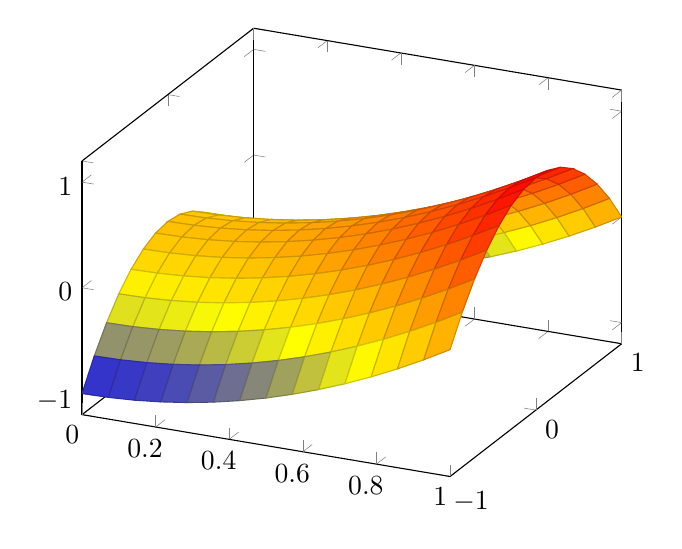
\begin{tikzpicture}
\begin{axis}
    \addplot3 [
	surf,
	samples=15,
	domain=0:1,y domain=-1:1
    ] {x^2 - y^2};
\end{axis}
\end{tikzpicture}
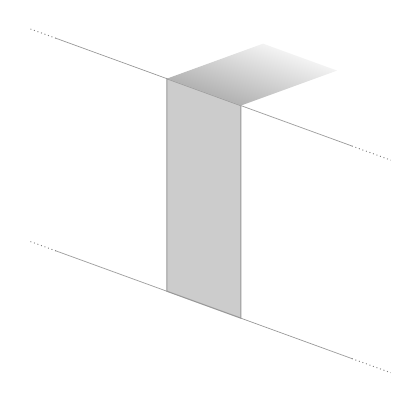
\begin{tikzpicture}[>=Stealth]
	\def\t{20}   		% angle
	\def\s{2}		% scale factor
	\def\h{\s*1.35}		% core height
	\def\l{\s*.5}		% core width
	\def\c{\s*.75}		% cladding width (before dots)
	\def\d{\s*.65}    	% depth
	\def\slw{.25pt}		% solid line width
	\def\dlw{.35pt}
	
	% Facing Box Coordinates
	\coordinate (a) at (0, 0);			% lower left
	\coordinate (b) at (-\t: \l);			% lower right
	\coordinate (c) at ($(-\t: \l)+(0, \h)$);	% upper right
	\coordinate (d) at (0, \h);			% upper left
	
	% Facing box and border
	\fill[gray!40]  (a) -- (b) -- (c) -- (d) -- cycle;  % Core region
	\draw[gray!80, thin]  (a) -- (b) -- (c) -- (d) -- cycle;
	
	% Right Cladding
	\draw[gray!80, line width=\slw] (b) -- +(-\t: \c);

	\draw[gray, densely dotted, line width=\dlw] (b) ++(-\t: \c) -- +(-\t:
		.35*\c);
	\draw[gray!80, line width=\slw] (c) -- +(-\t: \c);
	\draw[gray, densely dotted, line width=\dlw] (c) ++(-\t: \c) -- +(-\t: .35*\c);

	% Left cladding
	\draw[gray!80, line width=\slw] (a) -- +(-\t: -\c);
	\draw[gray, densely dotted, line width=\dlw] (a) ++(-\t: -\c) --
		+(-\t:-.25*\c);
	\draw[gray!80, line width=\slw] (d) -- +(-\t: -\c);
	\draw[gray, densely dotted, line width=\dlw] (d) ++(-\t: -\c) --
		+(-\t:-.25*\c);
	
	% Behind line
	% \draw[gray, thick, dotted] (b) -- +(\t: \d);
	
	% Top Box
	\shade[left color=gray!70, shading angle=-\t+180] (c) -- ++(\t: \d) --
	++(-\t: -\l) -- (d) -- cycle;
	
	% Axes
	% \draw[black!70, thick, ->] (d) ++(-\t: -.5*\c) -- +(-\t: -.65*\c) node[anchor=north east] {$x$};
	% \draw[black!70, thick, ->] (d) ++(-\t: -.5*\c) --+(0, .9*\c) node[anchor=east] {$y$};
    % \draw[black!70, thick, ->] (d) ++(-\t: -.5*\c) --+(\t: .65*\c) node[anchor=south] {$z$};
    
\end{tikzpicture}
\end{document}
